\hypertarget{a00331}{}\section{A\+A\+X Format Specification}
\label{a00331}\index{A\+A\+X Format Specification@{A\+A\+X Format Specification}}
Additional requirements for A\+A\+X plug-\/ins. 

This document describes aspects of the A\+A\+X plug-\/in format specification that are beyond the scope of the \hyperlink{a00325}{common interface classes and callbacks} that the plug-\/in must implement.

 \hypertarget{a00331_commoninterface_formatspecification__aaxplugin_directory_structure}{}\subsection{.\+aaxplugin Directory Structure}\label{a00331_commoninterface_formatspecification__aaxplugin_directory_structure}
A\+A\+X uses a bundle packaging format. On O\+S X, A\+A\+X plug-\/ins are built as standard O\+S bundles, while on Windows they are simple directories. All A\+A\+X plug-\/in bindles must use the .aaxplugin extension and the following directory structure\+:


\begin{DoxyItemize}
\item /\+Contents 
\begin{DoxyItemize}
\item /\+Resources 
\begin{DoxyItemize}
\item {\itshape This directory contains all of the additional resource files that will be needed by the plug-\/in at run time such as D\+S\+P algorithm D\+L\+Ls, X\+M\+L page tables, and image files for the plug-\/in\textquotesingle{}s G\+U\+I}  
\end{DoxyItemize}
\end{DoxyItemize}
\begin{DoxyItemize}
\item /\+Mac\+O\+S 
\begin{DoxyItemize}
\item {\itshape Contains the plug-\/in\textquotesingle{}s O\+S X binary (Mach-\/\+O)\textsuperscript{$\ast$}}  
\end{DoxyItemize}
\end{DoxyItemize}
\begin{DoxyItemize}
\item /\+Win32 
\begin{DoxyItemize}
\item {\itshape Contains the plug-\/in\textquotesingle{}s Windows x86 binary\textsuperscript{$\ast$}}  
\end{DoxyItemize}
\end{DoxyItemize}
\begin{DoxyItemize}
\item /x64 
\begin{DoxyItemize}
\item {\itshape Contains the plug-\/in\textquotesingle{}s Windows x64 binary\textsuperscript{$\ast$}}  
\end{DoxyItemize}
\end{DoxyItemize}
\begin{DoxyItemize}
\item /\+Factory Presets {\itshape (optional) } 
\begin{DoxyItemize}
\item {\itshape This directory includes built-\/in plug-\/in presets. For more information, see \hyperlink{a00360_subsection__presets_and_settings_management}{Presets and settings management} in the \hyperlink{a00360}{Pro Tools Guide} documentation}  
\end{DoxyItemize}
\end{DoxyItemize}
\begin{DoxyItemize}
\item Pkg\+Info {\itshape (O\+S X only) } 
\begin{DoxyItemize}
\item {\itshape This file must include the concatenation of the plug-\/in\textquotesingle{}s {\ttfamily C\+F\+Bundle\+Package\+Type} ({\ttfamily T\+D\+Mw}) and {\ttfamily C\+F\+Bundle\+Signature} ({\ttfamily P\+Tul})}  
\end{DoxyItemize}
\end{DoxyItemize}
\begin{DoxyItemize}
\item Info.\+plist {\itshape (O\+S X only) } 
\begin{DoxyItemize}
\item {\itshape The plug-\/in\textquotesingle{}s property list}  
\end{DoxyItemize}
\end{DoxyItemize}
\item desktop.\+ini (Windows only) 
\begin{DoxyItemize}
\item {\itshape The .aaxplugin directory\textquotesingle{}s view resource file, used to set its custom icon in Windows Explorer}  
\end{DoxyItemize}
\item Plug\+In.\+ico (Windows only) 
\begin{DoxyItemize}
\item {\itshape Custom plug-\/in icon file}  
\end{DoxyItemize}
\end{DoxyItemize}

\textsuperscript{$\ast$}See the following compatibility notes \begin{DoxyRefDesc}{Host Compatibility Notes}
\item[\hyperlink{a00380__compatibility_notes000003}{Host Compatibility Notes}]\begin{DoxyItemize}
\item The plug-\/in\textquotesingle{}s binary filename must be the same as the outer .aaxplugin bundle name \end{DoxyItemize}
\begin{DoxyItemize}
\item On Windows, the plug-\/in binary (D\+L\+L) must use the \char`\"{}.\+aaxplugin\char`\"{} suffix; i.\+e. the D\+L\+L must use exactly the same name as the outer .aaxplugin folder. On O\+S X, the plug-\/in binary does not require a specific suffix. \end{DoxyItemize}
\begin{DoxyItemize}
\item On Windows, the plug-\/in\textquotesingle{}s binary filename (and therefore also the outer .aaxplugin file name) must not contain any spaces. There is a bug in A\+A\+E that will prevent binaries with spaces from being loaded properly. This is logged as P\+T\+S\+W-\/189928.\end{DoxyItemize}
\end{DoxyRefDesc}


\begin{DoxyNote}{Note}
This directory structure is also used for plug-\/in installer directories in the V\+E\+N\+U\+E plug-\/in installer system. See \hyperlink{a00377_aax_venue_guide__installer}{V\+E\+N\+U\+E Plug-\/in installer specification} for more information.
\end{DoxyNote}


 \hypertarget{a00331_commoninterface_formatspecification__required_symbols}{}\subsection{Required Symbols}\label{a00331_commoninterface_formatspecification__required_symbols}
The following symbols are required in any A\+A\+X plug-\/in and must not be stripped from the binary\+: 
\begin{DoxyItemize}
\item {\ttfamily \+\_\+\+A\+C\+F\+Register\+Plugin } 
\item {\ttfamily \+\_\+\+A\+C\+F\+Register\+Component } 
\item {\ttfamily \+\_\+\+A\+C\+F\+Get\+Class\+Factory } 
\item {\ttfamily \+\_\+\+A\+C\+F\+Can\+Unload\+Now } 
\item {\ttfamily \+\_\+\+A\+C\+F\+Startup } 
\item {\ttfamily \+\_\+\+A\+C\+F\+Shutdown } 
\item {\ttfamily \+\_\+\+A\+C\+F\+Get\+S\+D\+K\+Version }\textsuperscript{$\ast$} 
\end{DoxyItemize}

\begin{DoxyRefDesc}{Host Compatibility Notes}
\item[\hyperlink{a00380__compatibility_notes000004}{Host Compatibility Notes}]\textsuperscript{$\ast$}{\ttfamily \+\_\+\+A\+C\+F\+Get\+S\+D\+K\+Version} is required for 64-\/bit A\+A\+X plug-\/ins only\end{DoxyRefDesc}


 Collaboration diagram for A\+A\+X Format Specification\+:
\nopagebreak
\begin{figure}[H]
\begin{center}
\leavevmode
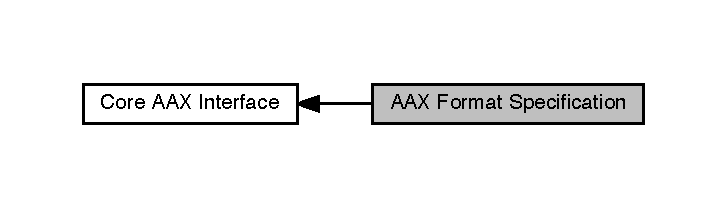
\includegraphics[width=349pt]{a00331}
\end{center}
\end{figure}
